\documentclass[pdflatex,11pt]{aghdpl}
% \documentclass{aghdpl}               % przy kompilacji programem latex
% \documentclass[pdflatex,en]{aghdpl}  % praca w języku angielskim
\usepackage[polish]{babel}
\usepackage[utf8]{inputenc}

% dodatkowe pakiety
\usepackage{hyperref}
\usepackage{url}
\hypersetup{
    colorlinks,
    citecolor=black,
    filecolor=black,
    linkcolor=black,
    urlcolor=black
}
\usepackage{enumerate}
\usepackage{listings}
\lstloadlanguages{TeX}

%moje pakiety
%zdjecia
\usepackage{wrapfig}
\usepackage{graphicx}

%testy sklady
\usepackage{lipsum}

\lstset{
  literate={ą}{{\k{a}}}1
           {ć}{{\'c}}1
           {ę}{{\k{e}}}1
           {ó}{{\'o}}1
           {ń}{{\'n}}1
           {ł}{{\l{}}}1
           {ś}{{\'s}}1
           {ź}{{\'z}}1
           {ż}{{\.z}}1
           {Ą}{{\k{A}}}1
           {Ć}{{\'C}}1
           {Ę}{{\k{E}}}1
           {Ó}{{\'O}}1
           {Ń}{{\'N}}1
           {Ł}{{\L{}}}1
           {Ś}{{\'S}}1
           {Ź}{{\'Z}}1
           {Ż}{{\.Z}}1
}

%---------------------------------------------------------------------------

\author{Ernest Jęczmionek}
\shortauthor{E. Jęczmionek}

\titlePL{Symulacje ewolucji koalicji mieszanych}
\titleEN{Simulations of evolution of mixed coalitions}

\shorttitlePL{Symulacje ewolucji koalicji mieszanych} % skrócona wersja tytułu jeśli jest bardzo długi
\shorttitleEN{Thesis in \LaTeX}

\thesistypePL{Praca inżynierska}
\thesistypeEN{Bachelor of Science Thesis}

\supervisorPL{prof. dr hab. Krzysztof Kułakowski}
\supervisorEN{Professor Krzysztof Kułakowski}

\date{2017}

\departmentPL{Katedra Inforatyki Stosowanej i Fizyki Komputerowej}
\departmentEN{Department of Applied Informatics and Computational Physics}

\facultyPL{Wydział Fizyki i Informatyki Stosowanej}
\facultyEN{Faculty of Physics and Applied Computer Science}

\acknowledgements{Serdecznie dziękuję \dots tu ciąg dalszych podziękowań np. dla promotora, żony, sąsiada itp.}



\setlength{\cftsecnumwidth}{10mm}

%---------------------------------------------------------------------------

\begin{document}

\titlepages

\tableofcontents
\clearpage

\chapter{Wprowadzenie}
\label{cha:wprowadzenie}

Teoria gier wielu osobom kojarzy się z opisem gier towarzyskich między dwojgiem graczy, lecz takie rozgrywki to rzadkość w naszym zróżnicowanym świecie, gdzie zwykle w grę ekonomiczną, społeczną czy polityczną angażuje się wielu uczestników. 
W niniejszej pracy zostaną umówione gry wieloosobowe o niepełnej informacji. W tym typie gier ważnym elementem strategii jest odpowiedni wybór koalicjantów. Oczywiście nie jest możliwe aby uwzględnić wszystkie czynniki mogące mieć wpływ na grę, ale zostaną przeanalizowane dwa równania ewolucyjne, które mogłyby sterować graczami oraz przeprowadzona będzie analiza ich stabilności. Modelami gry użytymi w niniejszej pracy będzie gra 3-osobowa oraz gra wieloosobowa, w której gracze będą ustawieni w okręgu. Symulację partii w przypadku gier 3-osobowych będą obrazowane jako trójwymiarowe funkcje prawdopodobieństwa, natomiast dla gier wieloosobowych jako funkcje prawdopodobieństwa od czasu dla poszczególnych graczy.
%---------------------------------------------------------------------------


!!!TEST CYTATÓW!!! \cite{Now06} \cite{Hof98} \cite{Str01} \cite{Qt} \cite{Tut} \cite{Sza} \cite{Fsmd} \cite{Crf}
\chapter{Opis teoretyczny}
\label{cha:opis_teor}

\section{Gra 3 osobowa}
\label{sec:3_gra}

\paragraph{O jakiej grze mówimy}

W niniejszej pracy będziemy skupiali się na grze 3-osobowej.Będziemy rozpatrywać tylko przypadki w których koalicja dwóch graczy wygrywa. Nie bierzemy pod uwagę sytuacji w których współpraca ze sobą wszystkich graczy mogłaby przynieść najlepsze korzyści. W tabelce wypłat rozważanej gry nie może pojawić się punkt równowagi wynikający ze strategii czystych. W rozważane przez nas grze celem gracza nie jest zdobycie jak największego zysku, lecz osiągnięcie jak największej liczby wygranych. Osoba znajdująca się poza koalicją przegrywa i wszyscy gracze mają taką samą wagę wyboru.

Będziemy rozważali dwa przypadki: zależnej i niezależnej rozgrywki. Przez rozgrywkę niezależną rozumiem grę w której wynik partii w żaden sposób nie zależy od innych prowadzonych gier. Grę w okręgu opisuję jako rozgrywkę zależną, gdyż wybór dokonany lokalnie przez gracza wpływa na wyniki wyniki sąsiednich gier lokalnych. W pierwszej części skupimy się na partiach niezależnych, a następnie wykonamy symulacje gier ze sobą powiązanych. W grach zależnych każdy gracz będzie rozgrywał partie z dwoma innymi graczami siedzącymi po obu jego stronach, będzie to przypominało grę w okręgu gdzie każdy z graczy może wybrać czy wstępuje w koalicję z swoim partnerem po prawej czy lewej stronie. W takiej sytuacji nie będzie możliwe granie z oboma partnerami. Będziemy w końcu zmuszeni wybrać z kim trzymamy stałą koalicję, a kogo odrzucimy. Wykluczamy możliwość jakiejkolwiek komunikacji między graczami poza obserwowaniem ich poprzednich zagrań. Model ten z pewnością będzie dużo bardziej dynamiczny, gdyż częstotliwości wybierania sojuszy będzie musiała zmienić zachowanie sojuszników naszych partnerów.

\section{Model partii}
OPISZ TROJKAT GRY Z PRAWD I ZROB RYSUNEK

\section{Równania standardowe}
\label{sec:r_stand}

\begin{equation} \label{eq:stand}
p_i += \alpha \cdot (1 - \frac{n_R}{nr_{games}} - \frac{n_L}{nr_{games}})
\end{equation}

\section{Równania replikatorów}
\label{sec:r_repli}

OPISAĆ SPOSÓB WYPROWADZENIA OBYDWU!!! I CZYNNIK ZMNIEJSZCZYJĄCY NA KRAŃCACH !!!

\begin{equation} \label{eq:repli}
p_i += \alpha \cdot (p_i \cdot (1 - p_i)) \cdot (1 - \frac{n_R}{nr_{games}} - \frac{n_L}{nr_{games}})
\end{equation}

\section{Ograniczenie prawdopodobieństwa}
\label{sec:ograniczenie}
Jak zauważyliśmy powyższe równania w łatwy sposób mogą wyjść poza przedział $<0,1>$. Aby temu zapobiec każda inkrementacja prawdopodobieństwa musi być obłożona funkcją ograniczającą. Każde nowo obliczone prawdopodobieństwo podawane jest jako parametr do funkcji $ogr$, a dopiero jej rezultat jest przypisywany poszczególnym graczom. Zdecydowałem się użyć następującej funkcji:
\begin{displaymath}
ogr(p_i) = \left\{
\begin{array}{ll}
1 & \text{jeżeli } p_i > 1 \\
p_i & \text{jeżeli } 1 \geq p_i \geq 0 \\
0 & \text{jeżeli } p_i < 0
\end{array} 
\right\}
\end{displaymath}

Zapewne naszą uwagę przykuł także parametr $\alpha$ obecny w powyższych równaniach. W pierwszym z nich użycie go jest konieczne, gdyż w przeciwnym przypadku szacowanie prawdopodobieństwa innych doprowadziłoby to zawiązania trwałych koalicji już po pierwszej partii. N oznacza zagranie w stronę zawododnika z wyższym numerem, natomiast P z niższym. Zapętla to się dla pierwszego i ostatniego gracza. Zobaczmy przykład dla równania standardowego, prawdopodobieństwa początkowego $\frac{1}{2}$ i $\alpha = 1$ zakładając że:
\begin{align*}
Gracz_0 = N, Gracz_1 = P, Gracz_2 = N && Gracz_0 = N, Gracz_1 = P, Gracz_2 = P\\
\left\{
\begin{array}{ll}
\Delta p_0 = (1 - 0 - 1) =  0 & p_0=\frac{1}{2}\\
\Delta p_1 = (1 - 1 - 1) =  -1 & p_1= 0\\
\Delta p_2 = (1 - 1 - 0) =  0 & p_2=\frac{1}{2}\\
\end{array} 
\right\} &&
\left\{
\begin{array}{ll}
\Delta p_0 = (1 - 0 - \frac{1}{2}) =  0 & p_0=\frac{3}{4}\\
\Delta p_1 = (1 - \frac{1}{2} - 1) =  -\frac{1}{2} & p_1= 0\\
\Delta p_2 = (1 - 0 - \frac{1}{2}) =  \frac{1}{2} & p_2=\frac{3}{4}\\
\end{array}
\right\}
\end{align*}
Jak widzimy prowadzi to do bardzo szybkich zmian prawdopodobieństwa, co może praktycznie uniemożliwiać jakiekolwiek zmiany sojuszy. Co jednak z równaniami replikatorów? Czy również tam potrzebny będzie nam jakiś parametr zmniejszający dynamikę? Przecież zawierają one człon postaci $x(1-x)$, czy to nie wystarczy? Weźmy założenia z poprzedniego przykładu. Przeanalizujmy przykład: 
\begin{align*}
Gracz_0 = N, Gracz_1 = P, Gracz_2 = N \\
\left\{
\begin{array}{ll}
\Delta p_0 = \frac{1}{2} \cdot (1 - \frac{1}{2}) \cdot (1 - 0 - 1) =  0 & p_0=\frac{1}{2}\\
\Delta p_1 = \frac{1}{2} \cdot (1 - \frac{1}{2}) \cdot (1 - 1 - 1) =  0 & p_1= \frac{1}{4}\\
\Delta p_2 = \frac{1}{2} \cdot (1 - \frac{1}{2}) \cdot (1 - 0 - 1) =  0 & p_2=\frac{1}{2}\\
\end{array} 
\right\}
\\
Gracz_0 = N, Gracz_1 = P, Gracz_2 = P \\
\left\{
\begin{array}{ll}
\Delta p_0 = \frac{1}{2} \cdot (1 - \frac{1}{2}) \cdot (1 - 0 - \frac{1}{2}) = \frac{1}{8} & p_0=\frac{5}{8}\\
\Delta p_1 = \frac{1}{4} \cdot (1 - \frac{1}{4}) \cdot (1 - \frac{1}{2} - 1) = -\frac{1}{32} & p_1= \frac{7}{32}\\
\Delta p_2 = \frac{1}{2} \cdot (1 - \frac{1}{2}) \cdot (1 - 0 - \frac{1}{2}) = \frac{1}{8}  & p_2=\frac{5}{8}\\
\end{array}
\right\}
\end{align*}
Jak widzimy najszybsza zmiana zachodzi dla pierwszego gracza, który traci 25\% zaufania do gracza o wyższym indeksie. W kolejnej partii nie widzimy już tak dużych zmian. Czy jest to na tyle dużo, aby wprowadzać parametr mający spowalniać dynamikę zmian? Zanim odpowiem chciałbym poruszyć dwie kwestie. Zgadzam się że dynamika prawdopodobieństwa jest dla mnie akceptowalna(czyli wynosi do 10\%), ale tylko dla prawdopodobieństw które oddalają się od środka przedziału, a grę rozpoczynamy właśnie w nim. Drugą sprawą jest porównanie obu równań. Porównanie wyników, w które rekurencyjnie wkładamy czynnik wymnażający zmianę nie jest najłatwiejszą rzeczą do opisania. Ale czy człon $x(1-x)$ w równaniu replikatorów nie jest takim czynnikiem? Owszem jest, ale ... właśnie jego celem jest rozwiązanie problemu supersilnych, szybko tworzących się koalicji.
Weźmy na tapet przypadek, gdy w jednej z partii żaden z graczy nie współpracował:

RYSUNKI

\chapter{Implementacja symulacji}
\label{cha:implementacja}

\section{Opis problemu}
\label{sec:opis_problemu}
Symulacja gry 3-osobowej będzie przedstawiona jako sześcian. Każdy z jego wierzchołków będzie miał współrzędną składającą się z kombinacji 0 i 1, co ma obrazować prawdopodobieństwo gracza. Odpowiednio prawdopodobieństwo gracza pierwszego przedstawia oś x, drugiego oś y, trzeciego oś z. Każda funkcja reprezentuje jedną instancję gry 3-osobowej. Rysowane funkcje będą przedstawiały prawdopodobieństwa graczy ($p_i$) wynikające z używanych równań i zachowania przeciwników. 

Symulacja gry N-osobowej, w której gracze ustawieni są w okręgu będzie obrazowana jako funkcje prawdopodobieństwa każdego gracza od numeru partii.
%-------------------------------------------------------------------------------------------------------------------------------------------------------------

\section{Środowisko QT}
\label{sec:qt}
Do stworzenia programu wykorzystano QT Creator IDE z kilku powodów, które zaraz zostaną rozwinięte. Najważniejszą cechą środowiska jest udostępnienie go na kilku rodzajach licencji, z czego użyta tu została licencji LGPL. Pozwala ona na darmowe użytkowanie i modyfikowanie plików źródłowych, lecz udostępnienie własnego programu musi odbyć się na tej samej licencji. Kolejnym ważnym elementem jest multiplatformowość pozwalająca w łatwy sposób przenosić kod programu między systemami operacyjnymi, o ile nie zostały użyte biblioteki dostępne tylko na jeden z systemów. Kolejną z zalet jest łatwy i intuicyjny interfejs tworzenia graficznego interfejsu użytkownika, osoba mająca wcześniej styczność z na przykład biblioteką Swing Java'y nie powinna mieć problemu z zaadaptowaniem się do  formularza QT Creatora. Używanie nowoczesnego języka C++ (w pracy użyto wersji 14) nie sprawia problemów. Przed użyciem klas z bibliotek standardowych C++ warto sprawdzić czy biblioteka QT nie zawiera specjalnych klas opakowujących je. Przykładem może być \texttt{pthread} i \texttt{QThread} \cite{Qt}.

%-------------------------------------------------------------------------------------------------------------------------------------------------------------

\section{Schemat programu}
\label{sec::schemat}
Rysunek \ref{fig:schemat} przedstawia poglądowy schemat działania programu\cite{Tut}. Dzieląc rysunek na lewą i prawą część możemy wyodrębnić dwa wątki. Po lewej wątek odpowiadający za wykonanie symulacji, po prawej wątek odpowiadający za rysowanie. Określeniem \textit{Zasób} są opisane współdzielone dane ( opisane w podrozdziale \ref{sec::kod}) między wątkami, którymi jest historia symulacji. 

Podczas startu programu zostaje narysowany sześcian, po czym program przechodzi w stan nasłuchiwania na sygnały. Przykładowymi sygnałami mogą być zmiana rozmiaru okna aplikacji, bądź obrót figury. Po wykryciu takowego, następują próby zablokowania dostępu do zasobu dopóki nie zostanie to wykonane (zasób może być zablokowany przez inny wątek). Następnie na podstawie historii symulacji i/lub sygnału dokonywane jest nowe rysowanie. Po czym zasób zostaje zwolniony, a główny wątek (odpowiedzialny za rysowanie) wraca do stanu nasłuchiwania. 
\begin{figure}
    \centering
    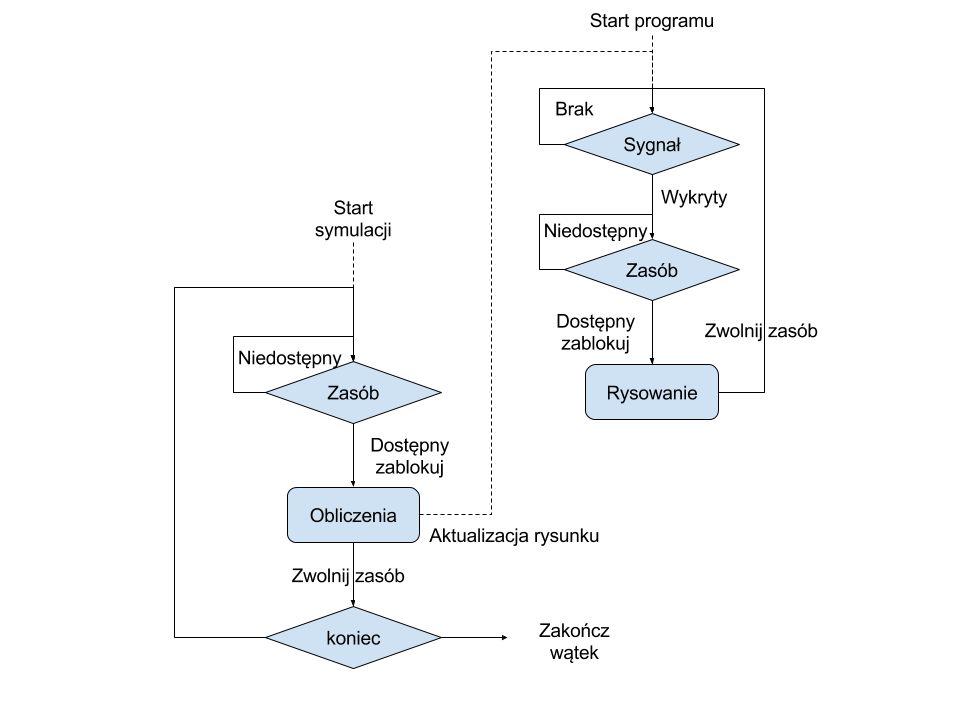
\includegraphics[width=0.9\textwidth]{pict/schemat.png}   
    \caption{Schemat programu}
	\label{fig:schemat} 
\end{figure}
Podczas startu symulacji (spowodowanej naciśnięciem przycisku \texttt{RUN}) identycznie jak poprzednio musi być uzyskany dostęp do zasobów. Dopiero po tym możliwe jest przeprowadzenie symulacji jednej partii dla każdej instancji gry. Następnie wyniki zostają zapisane do zasobów, po czym zasoby zostają zwolnione. Równocześnie do wątku głównego wysyłany jest sygnał mówiący o aktualizacji historii symulacji. Jeśli była to ostatnia planowana partia wątek symulacyjny kończy swoje działanie.
%-------------------------------------------------------------------------------------------------------------------------------------------------------------

\section{Sygnały, sloty i mutex}
\label{sec::sig_slot}
Komunikacja między klasami dziedziczącymi po \texttt{QObject} odbywa się przy pomocy połączonych ze sobą sygnałów i slotów \cite{Qt}. Można na nie patrzeć jako funkcje (sloty) oraz wskaźniki do funkcji (sygnały). Sygnał może trafiać do wielu slotów oraz do slotu może docierać wiele sygnałów. Ważne jest aby typy parametrów w deklaracji sygnału pokrywały się z typami parametrów deklaracji slotu. W przypadku gdy sygnał będzie miał zbyt dużo parametrów dla slotu, nadmiarowe parametry zostaną pominięte.

W celu uniknięcia kolizji zapis-odczyt na współdzielonych zasobach została użyta klasa \texttt{mutex} \cite{Crf}. Jest to semafor, nie chroni on danych przed dostępem z wielu źródeł, a jedynie informuje czy zasoby są obecnie używane czy nie. Nie ma niebezpieczeństwa wykonania operacji kolizyjnych, gdyż zasoby są wykorzystywane jedynie przez wewnętrzne struktury programu, które nie wykonują operacji na wspólnych zasobach jeśli semafor jest zablokowany.
%-------------------------------------------------------------------------------------------------------------------------------------------------------------

\section{Kod}
\label{sec::kod}
W tym podrozdziale będą opisane kluczowe fragmenty kodu, niezbędne do zrozumienia implementacji programu. Współdzielonymi zasobami są:
\begin{lstlisting}
template<typename T> using tup3= tuple<T,T,T>;
vector<vector<tup3<double>>> beginsp; //wektor historii punktów początkowych odcinków
vector<vector<tup3<double>>> endsp; //wektor historii punktów końcowych odcinków
vector<tup3<int>>colorsp; //kolory funkcji
mutex points;
\end{lstlisting}

\paragraph{Interfejs klasy \texttt{Game}}
Cała symulacja przeprowadzana jest w klasie \texttt{Game}, dlatego zostanie teraz omówiona. Reprezentuje ona jedną instancję gry 3-osobowej. Parametrem konstruktora jest indeks tablicy \texttt{decision\_funs}, której element zostaje przypisany do \texttt{decision}. \texttt{function} jest wrapperem biblioteki standardowej dla dowolnej funkcji, wyrażenia lambda, wyrażenia bind, funkcjonału lub wskaźników do funkcji. W poniższym kodzie \texttt{function} jest parametryzowany bezargumentowym, bezwynikowym zachowaniem. Funkcja \texttt{next} przeprowadza rozgrywkę jednej partii. Jej implementacja zostanie przedstawiona później. Zmienna \texttt{current} odpowiada $l_p$, natomiast \texttt{nr[i]} odpowiada $n_i$ (opisano w podrozdziale \ref{sec:model}). Funkcja \texttt{checker} jest odpowiednikiem funkcji $ogr$ (opisano w podrozdziale \ref{sec:ograniczenie}). Tablica \texttt{decision\_funs} zawiera funkcje lambda mające dostęp do prywatnych zmiennych klasy \texttt{Game}. W tablicach \texttt{result} znajdują się obliczone $\Delta p_i$, które następnie poddawane są funkcji ograniczającej. 

\begin{lstlisting}
class Game{
public:
    Game(int f);
    tup3<double> next();
    int getCurrent(); //zwraca numer bieżącej partii
    tup3<double> prelast(); //zwraca pre
private:
    array<double,3> p; //prawdopodobieństwa
    tup3<double> pre; //ostatnia krotka prawdopodobieństw na podstawie, których było dokonane losowanie sojuszników
    int current; //numer bieżącej partii
    array<int,3> nr;
    double checker(double r);
    function<void()> decision; //dokonuje modyfikacji prawdopodobieństw
    array<function<void()>,2>decision_funs={{
      [this](){//standardowe
        array<double,3> result= {
            0.1*( 1 - static_cast<double>(nr[1])/current - static_cast<double>(nr[2])/current),
            0.1*( 1 - static_cast<double>(nr[2])/current - static_cast<double>(nr[0])/current ),
            0.1*( 1 - static_cast<double>(nr[0])/current - static_cast<double>(nr[1])/current )
        };
        for(int i=0; i<3; i++)
            p[i]= checker(p[i]+result[i]);
      },
      [this](){//replikatorów
        array<double,3> result= {
            0.1*(p[0]*(1-p[0])*(1-static_cast<double>(nr[1])/current-static_cast<double>(nr[2])/current)),
            0.1*(p[1]*(1-p[1])*(1-static_cast<double>(nr[0])/current-static_cast<double>(nr[2])/current)),
            0.1*(p[2]*(1-p[2])*(1-static_cast<double>(nr[0])/current-static_cast<double>(nr[1])/current))
        };
        for(int i=0; i<3; i++)
            p[i]= checker(p[i]+result[i]);
      }
    }};
};
\end{lstlisting}

\paragraph{Implementacja \texttt{Game::next}}
Tablica \texttt{choices} zawiera losowe wartości dla każdego z zawodników, na podstawie których dokonywane jest losowanie sojusznika.
\begin{lstlisting}
tup3<double> Game::next(){
    pre= make_tuple(p[0],p[1],p[2]);
    current++;
    array<double,3> choices= {static_cast<double>(rand())/RAND_MAX, static_cast<double>(rand())/RAND_MAX, static_cast<double>(rand())/RAND_MAX};
    for(int i=0; i<3; i++)
        if(choices[i]<p[i])
            nr[i]++;
    decision();
    return make_tuple(p[0],p[1],p[2]);
}
\end{lstlisting}

\paragraph{Implementacja wątku symulującego} \texttt{QtConcurrent::run} jest funkcją uruchamiającą w osobnym wątku funkcję podaną jako parametr \cite{Qt}. Zwraca ona obiekt \texttt{QFuture}, który nie może przerwać lub wstrzymać wątku. Poprzez \texttt{beginsp.resize(p)} tworzony jest wektor posiadający p pustych elementów(wektorów krotek), ponieważ już w pierwszej partii będziemy potrzebować osobnego wektora dla każdej instancji gry. Natomiast \texttt{beginsp[i].reserve(g)} rezerwuje pamięć dla g partii, gdyby ta funkcja nie została użyta prawdopodobnie wystąpiłaby realokacja pamięci, w celu zapewnienia jej ciągłości. Przekładałoby się to na spowolnienie działania programu. Napisałem prawdopodobnie, ponieważ standard języka nie precyzuje ilości pamięci domyślnie rezerwowanej przez wektor, co jest zostawione po stronie implementacji. Przed wykonaniem każdej partii wątek czeka na dostęp do zasobu. Funkcja \texttt{try\_lock()} zwróci \texttt{true} w przypadku udanego przydzielenia zasobu, w przeciwnym razie zwróci \texttt{false}. 
\begin{lstlisting}
QtConcurrent::run(
            [&]()->void{
                ui->pushButton_Run->setEnabled(false);
                const int g= nr_rounds;
                const int p= nr_players;
                const int f= fun;
                vector<unique_ptr<Game>> tab;
                std::default_random_engine generator;
                std::uniform_int_distribution<int> distribution(0,255);
                auto r= bind(distribution, generator);
                clear_vectors();
                chrono::milliseconds d(delay);
                beginsp.resize(p);
                endsp.resize(p);
                for(int i=0; i<p;i++){
                    tab.push_back(make_unique<Game>(f));
                    colorsp.push_back(make_tuple( r(), r(), r() ));
                    beginsp[i].reserve(g);
                    endsp[i].reserve(g);
                }
                for(int j=0; j<g;j++){
                    if(quit) return;
                    while(!points.try_lock());
                    for(int i=0; i<p;i++){
                        beginsp[i].push_back(tab[i]->next());
                        endsp[i].push_back(tab[i]->prelast());
                    }
                    points.unlock();
                    emit copy();
                    this_thread::sleep_for(d);
                }
                ui->pushButton_Run->setEnabled(true);
            });
\end{lstlisting}

%-------------------------------------------------------------------------------------------------------------------------------------------------------------

\section{Rysowanie 3D}
\label{sec::3d}
\paragraph{Rysowanie}
Rysowanie sześcianu oraz funkcji zostało wykonane jako rysowanie odcinków. Ze względu na ograniczony krok czasowy symulacji funkcje wyglądają na wygładzone. Środek sześcianu jest środkiem układu współrzędnych.
\paragraph{Rozszerzanie}
Do rozszerzania ekranu został użyta następująca funkcja\cite{Tut} :
\begin{lstlisting}
void MyGLWidget::resizeGL(int width, int height){
    int side = qMin(width, height);
    glViewport((width - side) / 2, (height - side) / 2, side, side);
    glMatrixMode(GL_PROJECTION);
    glLoadIdentity();
#ifdef QT_OPENGL_ES_1
    glOrthof(-1, +1, -1, +1, 1.0, 15.0);
#else
    glOrtho(-1, +1, -1, +1, 1.0, 15.0);
#endif
    glMatrixMode(GL_MODELVIEW);
}
\end{lstlisting}
Oknem widgetu jest widoczny na ekranie prostokąt. Oknem roboczym widgetu jest obszar, na którym przeprowadzane są operacje. Oba okna nie muszą się pokrywać, mogą istnieć sytuacje, w których rysowane są elementy poza widokiem użytkownika. Posiadając żądane wymiary nowego okna należy wyznaczyć nowe położenie i wymiary nowego okna roboczego tak, aby zachować proporcje sześcianu oraz przedstawić go w całości. Argumentami funkcji \texttt{glViewport} są kolejno: współrzędne x i y lewego dolnego rogu widoku, szerokość i wysokość okna roboczego. Okno robocze musi być dopasowane do najkrótszego wymiaru widgetu, aby figury nie znalazły się poza oknem widgetu. Aby zapewnić wycentrowanie widoku roboczego należy dobrać punkt początkowy okna roboczego (lewy, dolny narożnik). Musi on mieć współrzędną punktu początkowego krótszej krawędzi jako 0, ponieważ chcemy wykorzystać ją całą. Współrzędna punktu początkowego dłuższej krawędzi okna roboczego musi być oddalona od punktu początkowego okna widgetu o połowę niewykorzystanej długości. Prowadzi to do wzoru na punkt początkowy okna roboczego: 
\begin{equation}
p_0=(\frac{1}{2}(\text{szerokość}-min(\text{szerokość}, \text{wysokość}),\frac{1}{2}(\text{wysokość}-min(\text{szerokość}, \text{wysokość}))
\end{equation}
Mając okno robocze o odpowiednich wymiarach zostało tylko przesunięcie układu współrzędnych do centrum okna roboczego przy pomocy funkcji \texttt{glOrtho}.
\paragraph{Obracanie}
\begin{wrapfigure}{rh}{0.2\textwidth}
    \centering
    \begin{tikzpicture}[scale=0.2]
		\tikzstyle{every node}+=[inner sep=0pt]
		\draw (34.9,-30) node {$(x_0,y_0)$};
		\draw (47.6,-23) node {$(x_1,y_1)$};
		\draw [black] (37.53,-28.55) -- (44.97,-24.45);
		\fill [black] (44.97,-24.45) -- (44.03,-24.4) -- (44.51,-25.27);
	\end{tikzpicture}
    \caption{Obrót - ruch myszy}
	\label{fig:obrot} 
\end{wrapfigure}
Kąt obrotu figury \cite{Tut} jest wyznaczany na podstawie punktu, gdzie klawisz myszy został wciśnięty $(x_0,y_0)$ oraz punktu w którym jest nadal wciśnięty $(x_1,y_1)$.
Lewy przycisk myszki ma priorytet nad prawym. Lewy przycisk myszy generuje obrót względem osi x i y o odpowiednio $\Delta$ y i $\Delta$ x stopni, natomiast prawy przycisk generuje obrót względem osi x i z o odpowiednio $\Delta$ y i $\Delta$ x stopni. Obrót jest ograniczony od $0^\circ$ do $360^\circ$, wartości poza tym zakresem są do niego sprowadzane poprzez operacje $\pm 360^\circ$ . Wymnażane delt przez czynnik mniejszy od 1 prowadzi do spowolnienia obrotu.


%-------------------------------------------------------------------------------------------------------------------------------------------------------------

\section{Makefile}
\label{sec::makefile}
Do rysowania wykresu funkcji prawdopodobieństw od numeru partii został użyty plik \texttt{Makefile}, który wykona kompilację, uruchomienie oraz narysowanie wykresu przy pomocy programu gnuplot. Aby uruchomić program należy podać argument: G - ilość partii do rozegrania oraz P - ilość graczy. Poniżej przykładowe polecenie do wykonania symulacji dla 100 partii rozegranych przez 20 zawodników.
\begin{verbatim}
make G=100 P=20
\end{verbatim}
Podanie nierealnych wartości nie da wyniku. Główną różnicą w implementacja gry N-osobowej jest funkcja \texttt{Game::next()}.
\begin{lstlisting}
void Multigame::next() {
    ...
    p[0]+= 0.1*(p[0]*(1-p[0])*(1-static_cast<double>(nr_r[1])/current-static_cast<double>(nr_r[players-1])/current));
    for(int i=1; i<players-1; i++)
        p[i]+= 0.1*(p[i]*(1-p[i])*(1-static_cast<double>(nr_r[i+1])/current-static_cast<double>(nr_r[i-1])/current));
    p[players-1]+= 0.1*(p[players-1]*(1-p[players-1])*(1-static_cast<double>(nr_r[0])/current-static_cast<double>(nr_r[players-2])/current));
}
\end{lstlisting}
Szacowanie prawdopodobieństw musi być wykonane w pętli, ze względu na nieznaną liczę graczy.
\chapter{Wyniki}
\label{cha:wyniki}

\section{Gry 3-osobowe}
\label{sec:N3nzal}

\paragraph{Równania standardowe}
\label{sec:r_stan}
\begin{wrapfigure}{rh}{0.5\textwidth}
    \centering
    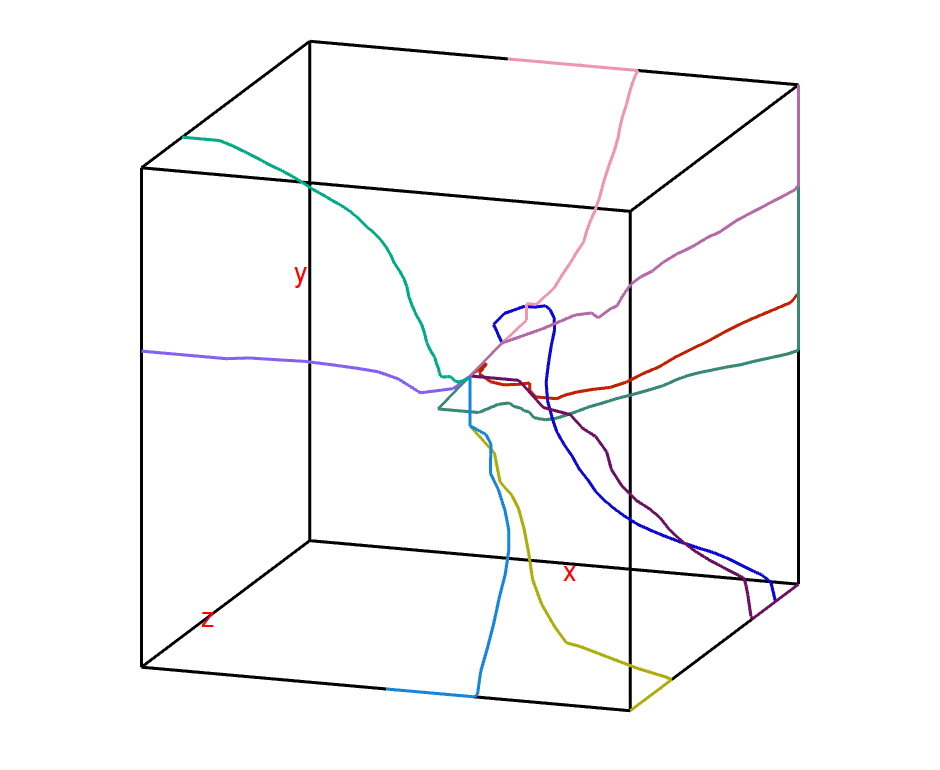
\includegraphics[width=0.5\textwidth]{pict/wyniki/stand100_10.png}   
    \caption{Równania standardowe: 50 gier, 10 graczy}
	\label{fig:stand50_10} 
\end{wrapfigure}

Postaramy się teraz przeanalizować wyniki symulacji z użyciem równań standardowych. Z analizy teoretycznej równań spodziewamy się zawiązania koalicji pomiędzy dwójką z graczy, wynikiem tego jest dążenie funkcji do krawędzi sześcianu. Po osiągnięcia trwałej koalicji trzeci gracz bezskutecznie stara się grać na jednego z koalicjantów. Jest to widoczne poprzez poruszanie się funkcji po krawędzi sześcianu dążącej do jego wierzchołków. Widać że funkcje idące od centrum zachowują się w miarę stabilnie idąc w kierunku jakiejś krawędzi nie zmieniają monotoniczności. Istnieją niewielkie wahania wynikające z prawdopodobieństwa, ale nie mają one większego wpływu w dążeniu do jednej z krawędzi i zmianę ich decyzji. 

Tak naprawdę koalicje zawiązują się tuż po zaczęciu gry i dążą bezpośrednio do stanu ustalonego,  ponieważ na początku gry szacowane prawdopodobieństwo u innych graczy jest bardzo duże. Wynika to z tego szacowane prawdopodobieństwo w pierwszej grze wynosi 0\% albo 100\% co definitywnie wskazuje aby grać na jednego z zawodników. Było to powodem dla którego wprowadziłem współczynnik $\alpha$ równy 0.1, który ma za zadanie blokować sytuacje w których od razu po pierwszej grze jesteśmy w trwałej koalicji.

Jeśli chcielibyśmy uzyskać szybszą grę powinniśmy używać większych współczynników $\alpha$, co skutkować będzie mniejszą szansą na zerwanie koalicji. Jeśli natomiast chcielibyśmy żeby gra przebiegała wolniej moglibyśmy obniżyć współczynnik $\alpha$, co doprowadziłoby do większej liczby zmian partnerów.


%\lipsum[1-5]

%---------------------------------------------------------------------------------------------------------------------------------------------------------
\paragraph{Równania replikatorów}
\label{sec:r_repl}

\begin{figure}
	\centering
	\begin{tabular}{c|c}
		\centering
		\subfloat[50 gier \label{fig:repl50_10}]{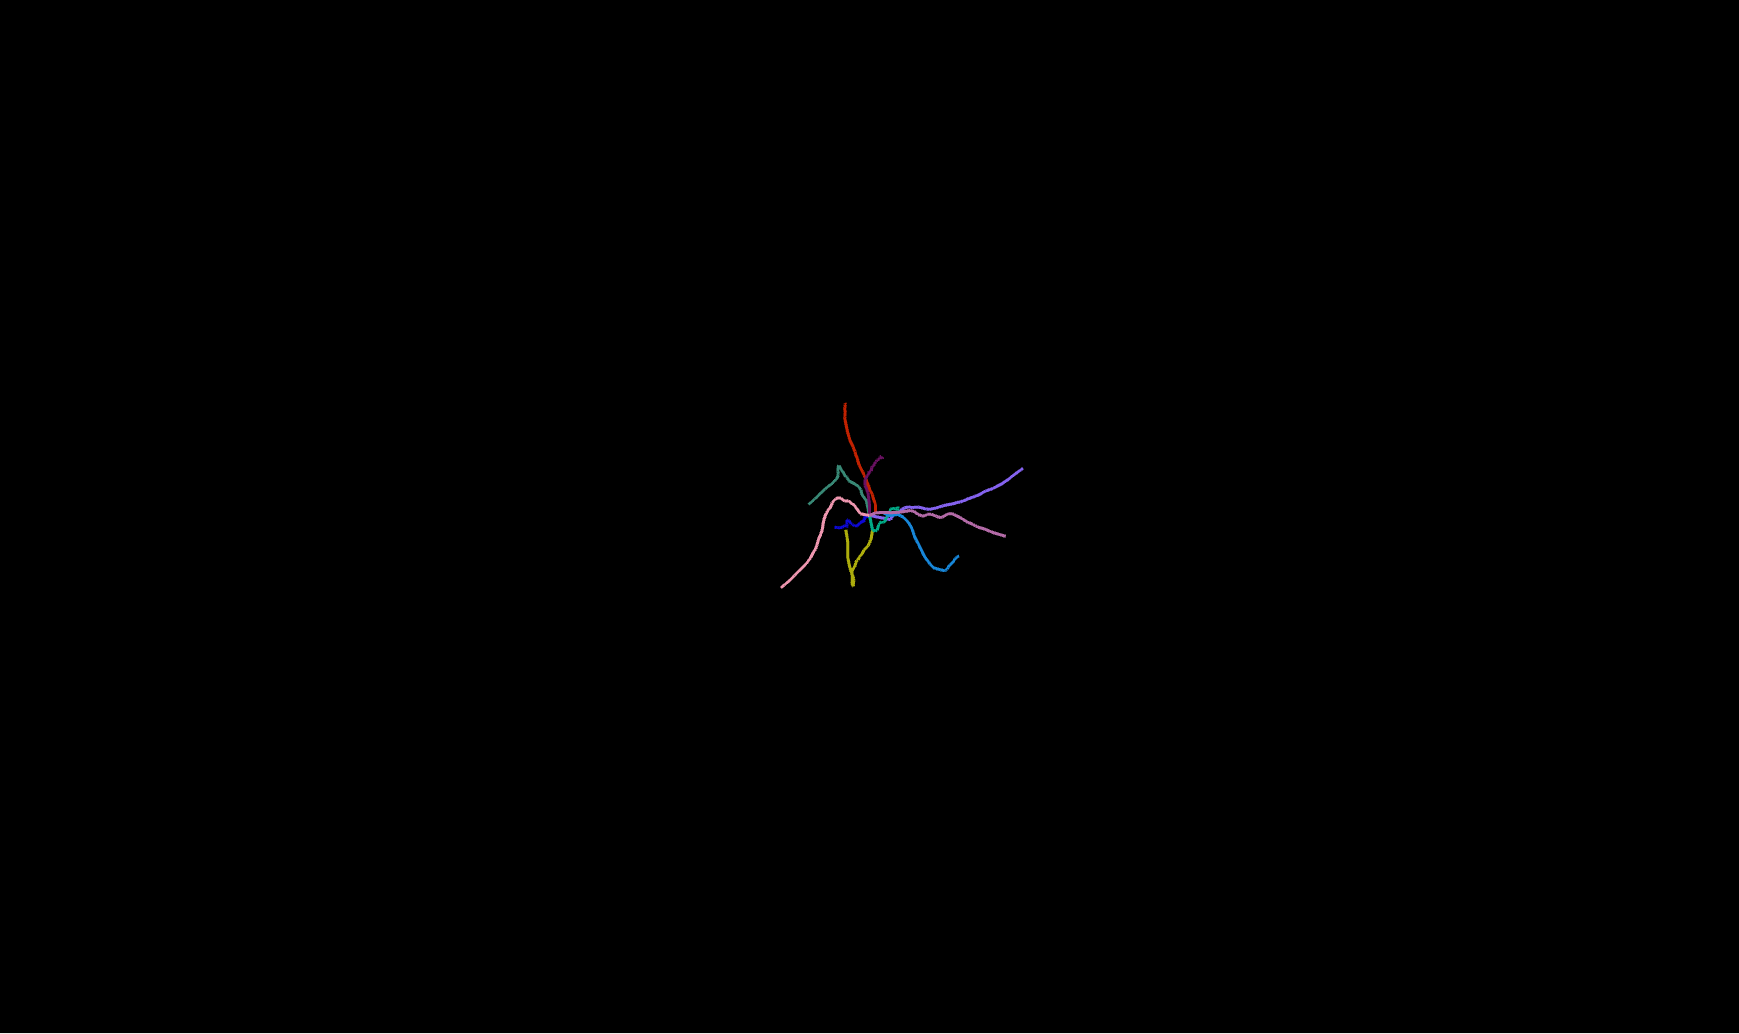
\includegraphics[width=.45\textwidth]{pict/wyniki/repl50_10.png}} 
		&
		\subfloat[250 gier \label{fig:repl250_10}]{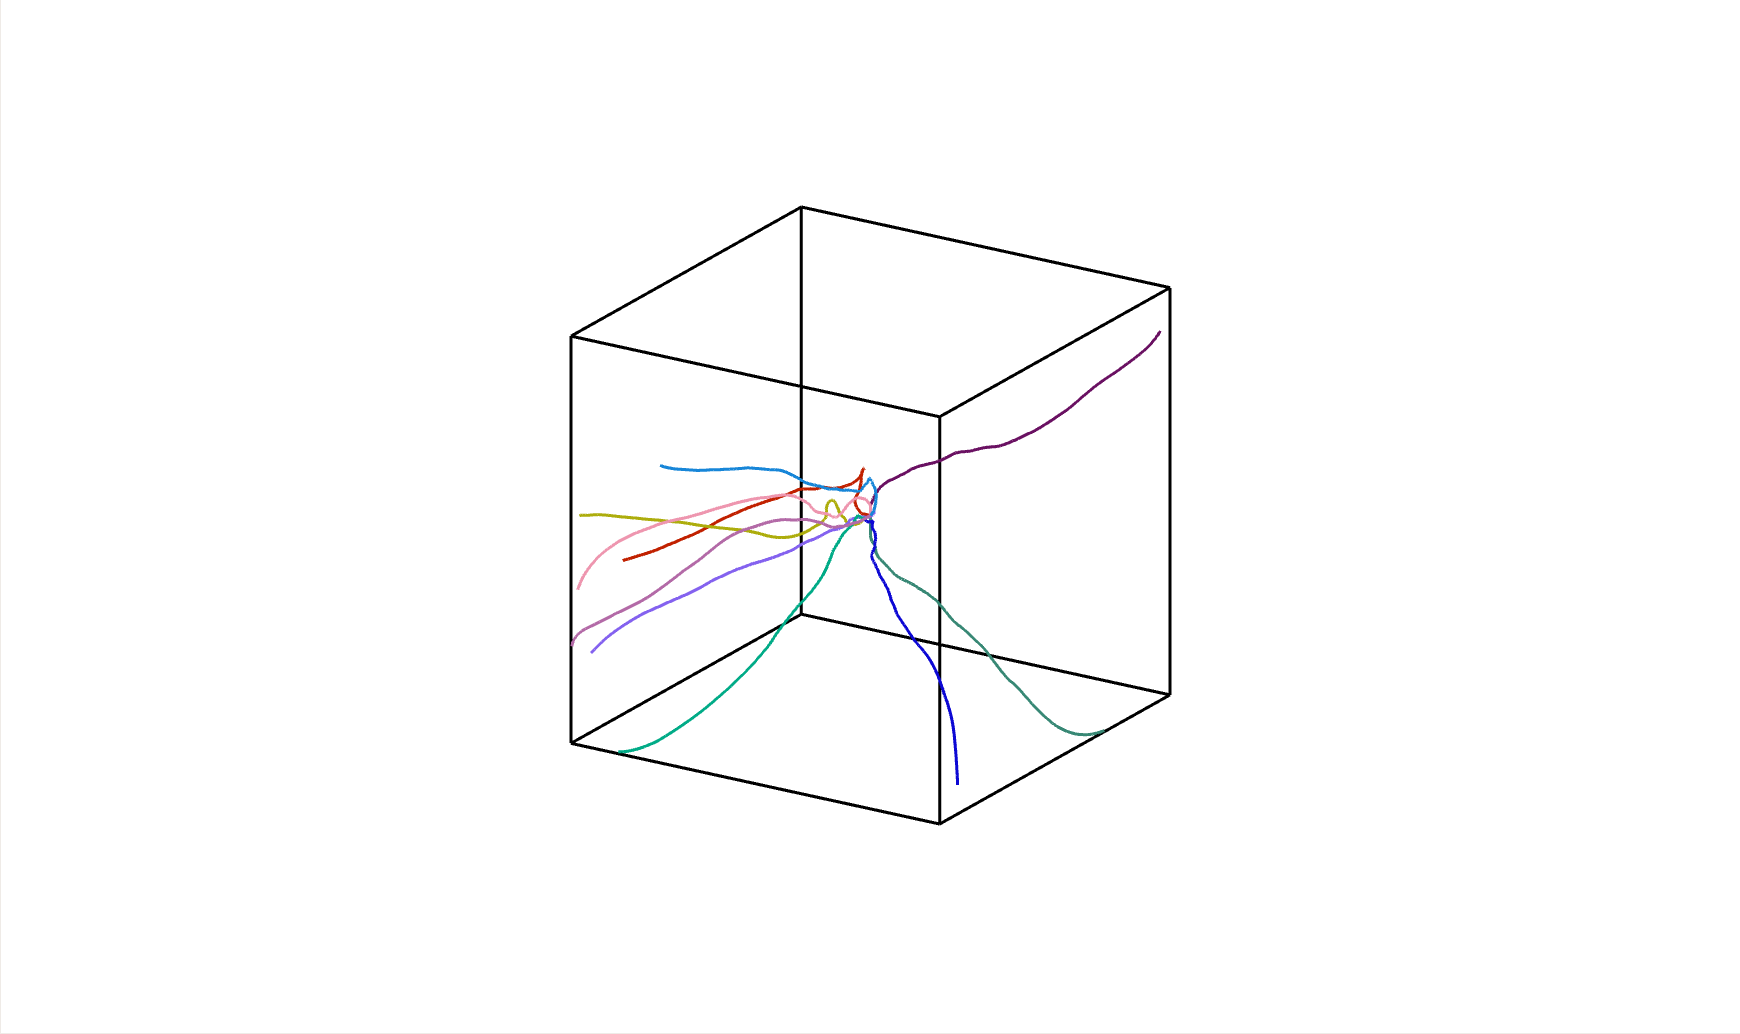
\includegraphics[width=.45\textwidth]{pict/wyniki/repl250_10.png}}
		\\ \hline
		\subfloat[1000 gier \label{fig:repl1000_10}]{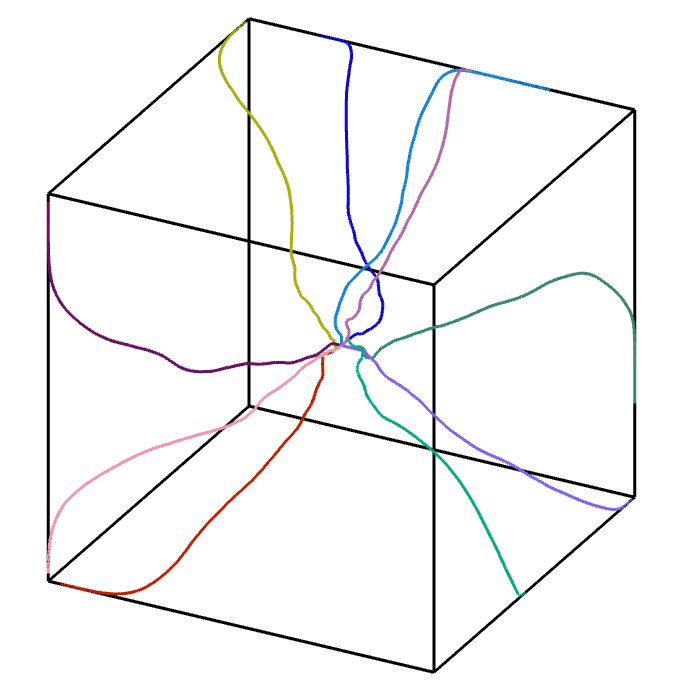
\includegraphics[width=.45\textwidth]{pict/wyniki/repl1000_10.png}}
		&
		\subfloat[10000 gier \label{fig:repl10000_10}]{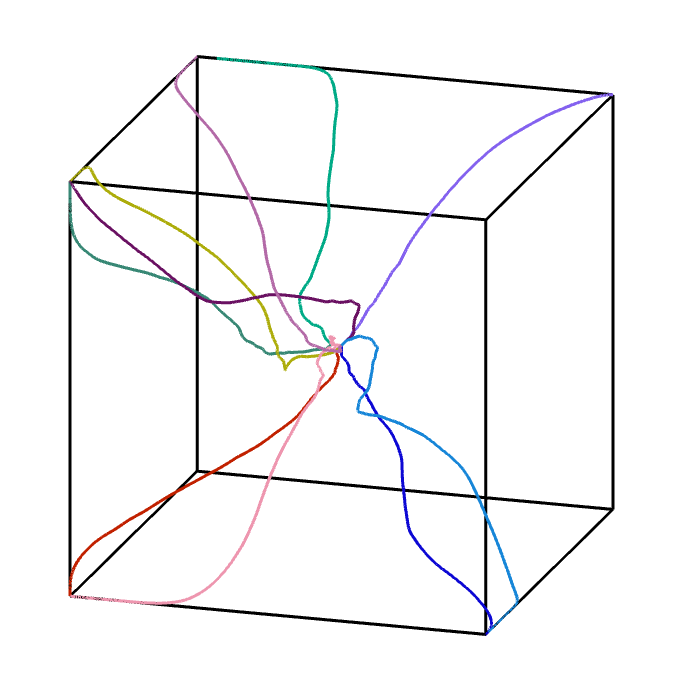
\includegraphics[width=.45\textwidth]{pict/wyniki/repl10000_10.png}}
	\end{tabular}
\caption{Równania replikatorów: 10 graczy}
\label{fig:repl_10}
\end{figure}

Od równania tego rodzaju spodziewamy się mniejszego wkładu, a jest to spowodowane tym że człon z własnym prawdopodobieństwem jest funkcja kwadratową $x(1-x)$ której maksimum ma wartości 0.5 i wynosi ono 0.25. Na krańcach dziedziny funkcji $<0,1>$ przyjmuje wartość 0 (przypomina wielomian węzłowy Lagrange'a). Co jest znacznym ograniczeniem dynamiki funkcji w stosunku do równań standardowych. Dobrym tego przykładem jest rysunek \ref{fig:repl50_10} na którym widać jak dla 50 gier prawdopodobieństwa zachowujemy się dużo wolniej w porównaniu z równaniami standardowymi co jest bezpośrednim wynikiem omawianego członu. Ograniczenie zmiany prawdopodobieństwa wprowadza możliwość zmiany koalicji, ponieważ prawdopodobieństwo przejścia między koalicjami wzrasta ze spadkiem maksymalnej pojedynczej jego zmiany. Widoczne na rysunku \ref{fig:repl50_10} kiedy to w początkowej fazie kilka koalicji rozwiązuje się i zmieniają partnerów, co nie było widoczne dla równań standardowych. Na rysunku \ref{fig:repl250_10} widzimy że tak samo jak dla równania standardowych i w tym przypadku funkcje prawdopodobieństwa dążą do krawędzi sześcianu, jednak dzieje się to znacznie wolniej gdyż człon równania z własnym prawdopodobieństwem dąży do 0. Dopiero dla 1000 gier zaczynamy obserwować sytuację podobną do 50 gier dla równań standardowych kiedy to funkcje prawdopodobieństwa dochodzą do krawędzi sześcianu i jeden z osamotniony graczy za wszelką cenę stara się grać tylko na jednego z partnerów aby wybić go ze stanu równowagi, co prowadzi do zmierzania do wierzchołków sześcianu, gdzie stan ustalony wygląda jako koalicja dwóch graczy z jednym wyobcowanym zawodnikiem, który jest zdecydowany na grę z jednym graczem lecz partner nie odwzajemnia jego chęci. Aż 10000 gier było wymagane aby prawdopodobieństwa doszły do wierzchołka gdzie mamy wcześniej opisaną sytuację.
%\lipsum[1-5]

%---------------------------------------------------------------------------------------------------------------------------------------------------------
\section{Gry N-osobowe}
\label{sec:N3zal}
\begin{wrapfigure}{rh}{0.5\textwidth}
    \centering
    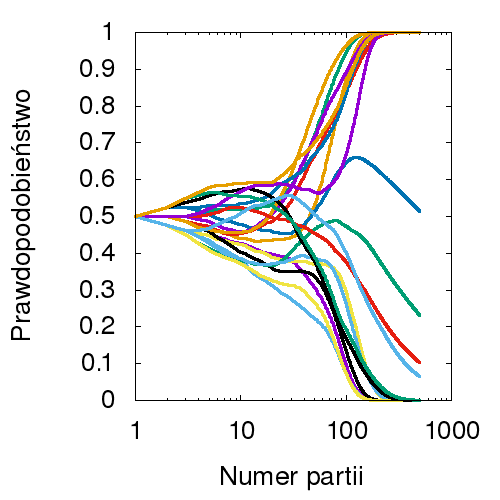
\includegraphics[width=0.5\textwidth]{pict/wyniki/g500p20}   
    \caption{Gra w okręgu: 500 gier, 20 graczy}
	\label{fig:podst} 
\end{wrapfigure}

Chciałbym teraz przeanalizować wyniki jednej z symulacji \ref{fig:podst}. Jak już wcześniej zaobserwowaliśmy równania replikatorów dają dużo mniejszą dynamikę decyzji graczy.

Peleton graczy tworzy stabilne koalicje około 300 partii które nie są w stanie ulec zmianie. Pozostałe przypadki tworzą niestabilne koalicje, które zmieniają się w czasie. Najlepszym tego przykładem jest gracz który początkowo gra w kierunku swojego prawego sąsiada, a później zapewne przez jego niechęć po kilku fluktuacjach zaczyna drastycznie zmieniać partnera swojej gry - zaznaczonych kolorem fioletowym. Czynnik losowy graczy utrudnia grę tylko z jednym wybranym partnerem, dlatego jak widzimy podczas pierwszych 50 gier dochodzi do dużej liczby zmian zachowań graczy. Szczególnie widoczne jest to w pierwszych 50 partiach, gdzie gracze dopiero szacują zachowanie sąsiadów. W kolejnych 50 partiach gracze zachowują się coraz bardziej liniowo, gdyż błąd przewidywanego i realnego prawdopodobieństwa przeciwnika spada. Nie wchodzący w stałą koalicja mogą należeć do łańcucha graczy niezdecydowanych lub jednostek znajdujących się pomiędzy dwoma silnymi koalicjami które nie dają szansy na przyłączenie się do żadnej. Wartym zauważenia jest fakt że ostatnia zmiana monotoniczności funkcji zachodzi dopiero około 300 gry.

\begin{wrapfigure}{rh}{0.5\textwidth}
    \centering
    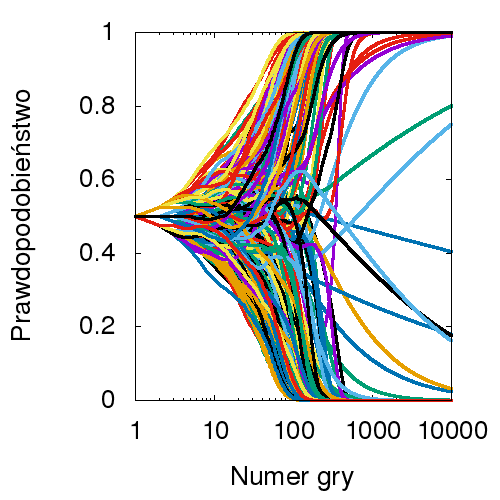
\includegraphics[width=0.5\textwidth]{pict/wyniki/g10000p200}   
    \caption{Gra w okręgu: 10000 gier, 200 graczy}
	\label{fig:niechciani} 
\end{wrapfigure}

Rozpatrzmy teraz dużo dłuższą grę w której zaangażowanych jest więcej graczy, co może pokazać nam przypadki szczególne. Na rysunku widzimy że większość zawodników osiąga stabilne koalicję przed grą 1000. Występuje grupka kilku graczy którzy pomimo tak dużej ilości gier nie byli w stanie zawiązać trwałych koalicji.

Mogło to wynikać z dwóch faktów. Po pierwsze mogli znaleźć się między graczami znajdującymi się w trwały w sojuszach którzy nie byli zainteresowani wchodzeniem w nowe. Drugą przyczyną może być nieznajomość prawdziwego prawdopodobieństwa podejmowania decyzji przez sąsiadów które jest tylko wartością znaną z rozgrywki różnica pomiędzy faktycznym prawdopodobieństwem gry sąsiada a tym co reprezentował. W rozgrywce może się znacząco różnić wpływając na mylną ocenę prawdopodobieństwa gry zawodników i mogących ustalić stabilnej koalicji. Rysunek \ref{fig:niechciani} pokazuje przypadek w którym dwóch silnych koalicjantów nie jest zainteresowanych wejście w sojusz z osamotnionym zawodnikiem między nimi, który jak widać z tabelki !!!REF!!! ZRÓB TABELKĘ !!! powoli próbuje dążyć do stałej koalicji z jednym z graczy.  


\chapter{Podsumowanie}
\label{cha:podsumowanie}

Celem pracy było przeprowadzenie symulacji  powstawania koalicji przez stosowanie strategii mieszanych. Oczekiwane wyniki na podstawie analizy matematycznej nie odpowiadały ściśle wynikom uzyskanym z symulacji. W metodach analitycznych zakłada się bowiem pełną informację graczy, podczas gdy w symulacji zakładano grę o niepełnej informacji. 

W celu zmniejszenia błędu szacowanego prawdopodobieństwa, można by uwzględniać do niego jedynie k-ostatnich gier. Spowodowałoby to trafne szacowanie prawdopodobieństwa podczas monotonicznej gry przeciwników w k partiach, czego skutkiem byłyby punkty stabilne na krawędziach po przeprowadzeniu na nich k partii. W niniejszej pracy szacowane prawdopodobieństwa nie mają możliwości dojścia do 0 lub 1, jeśli decyzje przeciwników nie były monotoniczne przez całą grę. Skutkiem tego jest przemieszczanie się funkcji po krawędziach sześcianu, co mogłoby ustać po k partiach jeśli tylko one uwzględniane byłyby w szacowaniu. Oczywiście szybkość poruszania się po krawędziach spada z czasem, lecz nigdy nie dojdzie do sytuacji w której spadnie do 0. Szacowanie prawdopodobieństw na podstawie tylko niektórych partii rodzi problem natury doboru wartości parametru k. 

Zgodnie z analizą funkcje dążyły do krawędzi sześcianu, omijając punkty niestabilne oraz krawędzie reprezentujące niemożliwe do zawiązania koalicje zgodnie z rysunkiem \ref{fig:szescian}.

Symulacje gier N-osobowych pokazały dążenie graczy do trwałych koalicji. Wartą przeanalizowania byłaby sytuacja losowej zmiany prawdopodobieństw części graczy w stanie ustalonym. Mogłoby to z czasem doprowadzić ustalenia nowego stanu ustalonego.

Używana tu metoda zastosowania koncepcji strategii mieszanych do określania koalicji jest owocem dyskusji autora z promotorem tej pracy.



% itd.
% \appendix
% \include{dodatekA}
% \include{dodatekB}
% itd.


\listoffigures

\bibliographystyle{alpha}
\bibliography{bibliografia}
%\begin{thebibliography}{1}
%
%\bibitem{Dil00}
%A.~Diller.
%\newblock {\em LaTeX wiersz po wierszu}.
%\newblock Wydawnictwo Helion, Gliwice, 2000.
%
%\bibitem{Lam92}
%L.~Lamport.
%\newblock {\em LaTeX system przygotowywania dokumentów}.
%\newblock Wydawnictwo Ariel, Krakow, 1992.
%
%\bibitem{Alvis2011}
%M.~Szpyrka.
%\newblock {\em {On Line Alvis Manual}}.
%\newblock AGH University of Science and Technology, 2011.cccccc
%\newblock \\\texttt{http://fm.ia.agh.edu.pl/alvis:manual}.
%
%\end{thebibliography}

\end{document}
